\chapter{Dimensionality Reduction}
    \section{Curse of Dimensionality}
        La Maledizione della Dimensionalità ($\textbf{Curse of Dimensionality}$) si riferisce a una serie di problemi che sorgono quando si lavora con dati ad alta dimensione.
        \\[1\baselineskip]
        La dimensione di un set di dati corrisponde al numero di attributi/features che esistono in un set di dati.
        Un set di dati con un numero elevato di attributi, generalmente dell'ordine di un centinaio o più, viene definito dati ad alta dimensione.
        \\[1\baselineskip]
        Alcune delle difficoltà che derivano dai dati ad alta dimensione si manifestano durante l'analisi o la visualizzazione dei dati per identificare i modelli, e alcune si manifestano durante l'allenamento dei modelli stessi.
        \\[1\baselineskip]
        All'aumentare della dimensionalità, il numero di punti richiesti per una buona prestazione di qualsiasi algoritmo aumenta in modo esponenziale.
        Il motivo è che avremmo bisogno di un numero sempre più grande di punti per una data combinazione di features, affinché qualsiasi modello di apprendimento sia valido.

        \begin{figure}[h]
            \caption{Relazione tra Performance e Dimensionalità}
            \centering
            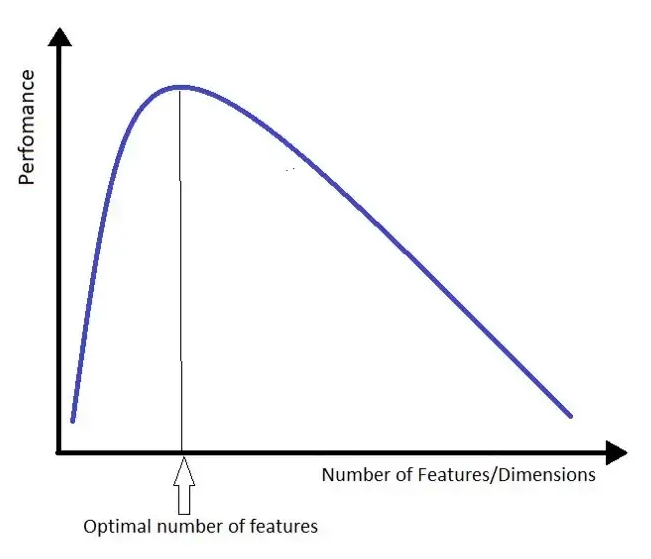
\includegraphics[width = 10cm]{dimensionality-curse-curve.png}
        \end{figure}

    \clearpage

    \section{PCA: Principal Component Analysis}
        L'analisi delle componenti principali, o $\textbf{PCA}$, è un metodo per la riduzione della dimensionalità che viene spesso utilizzato per ridurre la dimensionalità di set di dati di grandi dimensioni, trasformando un set di variabili di grandi dimensioni in uno più piccolo che contiene ancora la maggior parte delle informazioni nel set di dati originale.
        \\[1\baselineskip]
        La riduzione del numero di variabili di un set di dati va naturalmente a scapito dell'accuratezza, ma il trucco nella riduzione della dimensionalità è scambiare un po' di accuratezza con la semplicità: proprio perché i set di dati più piccoli sono più facili da esplorare e visualizzare, rendono l'analisi dei dati molto più semplice e veloce per gli algoritmi.
        \\[1\baselineskip]
        Quindi, per riassumere, l'idea di PCA è semplice: ridurre il numero di variabili di un set di dati, preservando quante più informazioni possibili.

        \subsection{Funzionamento}
            $\textbf{Nota:}$ non sono state elencate tutte a lezione, ma vengono lo stesso inserite (per completezza).
            \\[1\baselineskip]
            La PCA può essere suddivisa in cinque steps:

            \begin{enumerate}
                \item Standardizzare l'intervallo di variabili continue;
                \item Calcolare la matrice di covarianza/correlazione per identificare le correlazioni;
                \item Calcolare gli autovettori e gli autovalori della matrice di covarianza per identificare le componenti principali;
                \item Crea un vettore di caratteristiche per decidere quali componenti principali mantenere;
                \item Esegue un recasting dei dati lungo gli assi delle componenti principali.
            \end{enumerate}
        
            PCA trova le direzioni ortogonali della varianza massima dei dati forniti.
            Può essere pensato come una trasformazione in un nuovo sistema di coordinate, dove la prima coordinata (la prima componente principale) identifica la proiezione di massima varianza, la seconda coordinata la seconda massima varianza, etc...
            \\[1\baselineskip]
            Matematicamente, i componenti principali sono gli autovettori della matrice di covarianza.

            \begin{figure}[h]
                \caption[short]{Esempio di PCA}
                \centering
                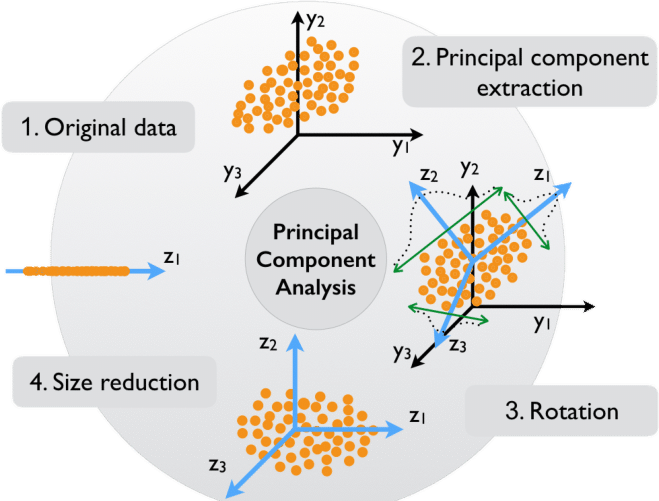
\includegraphics[width = 10cm]{PCA-example.png}
            \end{figure}
        
        \clearpage

        \subsection{Come trova le Componenti Principali?}
            Poiché ci sono tante componenti principali quante sono le variabili nei dati, le componenti principali sono costruite in modo tale che la prima componente principale rappresenti la massima varianza possibile nel set di dati.
            \\[1\baselineskip]
            $\textbf{Nota:}$ oltre alla massimizzazione della varianza (nell'esempio sottostante, la distanza fra i punti blu), si cerca anche di minimizzare la perdita di informazione (distanza tra la componente e i punti arancioni).
            
            \begin{figure}[h]
                \centering
                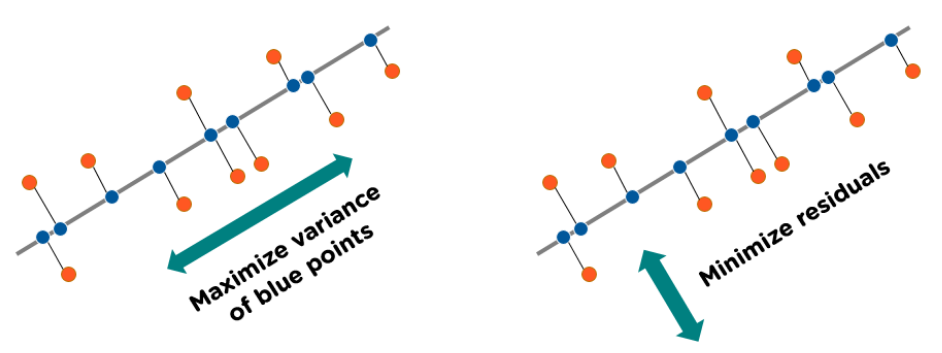
\includegraphics[width = 10cm]{PCA-example2.png}
            \end{figure}
            
            La seconda componente principale viene calcolata allo stesso modo, con la condizione che sia incorrelata con (cioè perpendicolare a) la prima componente principale e che tenga conto della successiva varianza più alta.
            Questo continua fino a quando non è stato calcolato un totale di $d$ componenti principali, pari al numero originale di variabili.
            \\[1\baselineskip]
            Alla fine del procedimento, i primi $m$ componenti con $m \le d$ ($d$ è la dimensione iniziale del dataset) diventeranno le nuove dimensioni del nuovo set di dati.

            \begin{figure}[h]
                \centering
                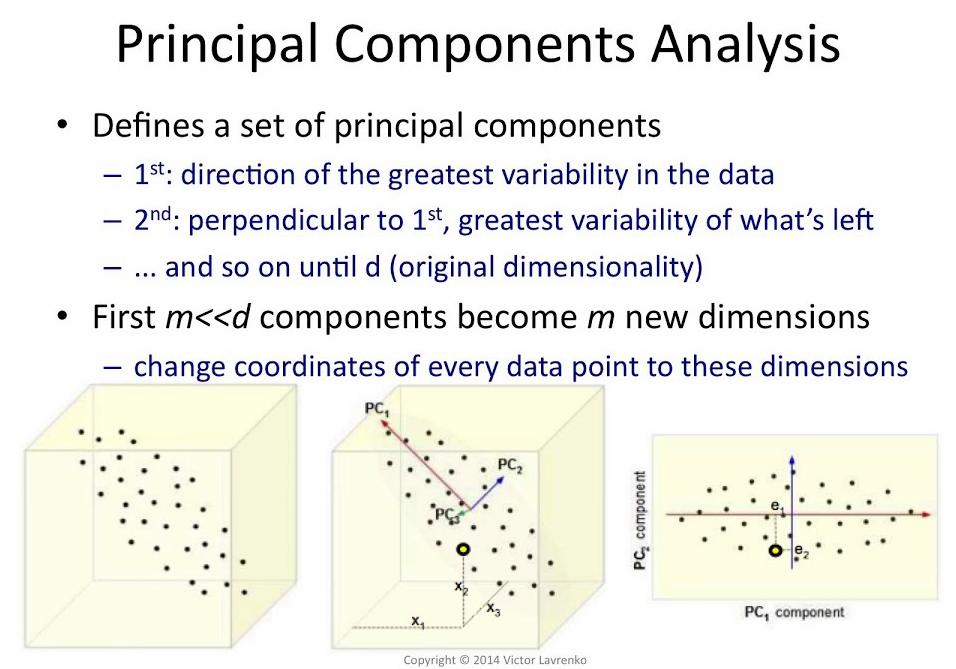
\includegraphics[width = 10cm]{PCA-explanation.jpg}
            \end{figure}

        \clearpage